% Results section (Part D, Milestone 6)
% Include from reports/midsem/main.tex (needs \usepackage{graphicx}).
%
% Every number below comes from a file written by a script or notebook:
%   results/metrics/err_mag_m.csv            python scripts/train_eval.py
%   results/metrics/err_mag_m_cv.csv         (same run; CV error per block)
%   results/diagnostics/alpha_sweep_err_mag_m.csv   python scripts/alpha_sweep.py
%   results/diagnostics/tuning_check_err_mag_m.csv  python scripts/tuning_check.py
%   results/diagnostics/window_length_ceiling.csv   python scripts/window_length_ceiling.py
%   segment and Lasso-weight numbers         notebooks/06 and notebooks/05
% The source is named in a comment above each table or paragraph. All numbers
% are for 2 s windows on MH_01_easy and MH_02_easy. Figure paths are relative
% to reports/midsem/.

\section{Results}
\label{sec:results}

All scores are on the held-out flight of each fold
(Section~\ref{sec:protocol}); the target is \texttt{err\_mag\_m} and the inputs
are the 104 Part~C features.

\subsection{Held-out performance}
\label{sec:results-heldout}

% Source: results/metrics/err_mag_m.csv (columns mae, r2; "mean" rows = average of the two folds)
\begin{table}[htbp]
\centering
\caption{Held-out MAE and $R^2$ for \texttt{err\_mag\_m}, by test flight.
The model is trained on the other flight.}
\label{tab:heldout}
\begin{tabular}{lrrrrrr}
\hline
 & \multicolumn{3}{c}{MAE (cm)} & \multicolumn{3}{c}{$R^2$} \\
Model & MH\_01 & MH\_02 & Mean & MH\_01 & MH\_02 & Mean \\
\hline
Mean baseline & 4.40 & 4.65 & 4.53 & $-0.04$ & $-0.02$ & $-0.03$ \\
OLS           & 3.12 & 2.87 & 2.99 & 0.40 & 0.76 & 0.58 \\
Ridge (L2)    & 2.80 & 2.60 & 2.70 & 0.63 & 0.80 & 0.72 \\
Lasso (L1)    & 2.59 & 2.42 & 2.50 & 0.68 & 0.84 & 0.76 \\
\hline
\end{tabular}
\end{table}

Table~\ref{tab:heldout} gives the headline result. Every model beats the mean
baseline on both flights. Lasso is best in both folds: its mean MAE of 2.50\,cm
is 45\% below the baseline's 4.53\,cm, and it explains 76\% of the test flight's
drift variation on average. Ridge is close behind (2.70\,cm, $R^2 = 0.72$);
OLS gains least (2.99\,cm, $R^2 = 0.58$) and is weakest on MH\_01
($R^2 = 0.40$), where it is trained on the shorter flight.
% Source: results/metrics/err_mag_m.csv (columns rmse, bias, "mean" rows)
RMSE gives the same order (fold means: baseline 6.91, OLS 4.15, Ridge 3.49,
Lasso 3.23\,cm), and all models are nearly unbiased: the largest mean bias is
$-0.49$\,cm (OLS), and Lasso's is $-0.12$\,cm. The baseline's bias is
$\pm 1.17$\,cm per fold because the two flights' mean drifts differ by that much.

\begin{figure}[htbp]
\centering
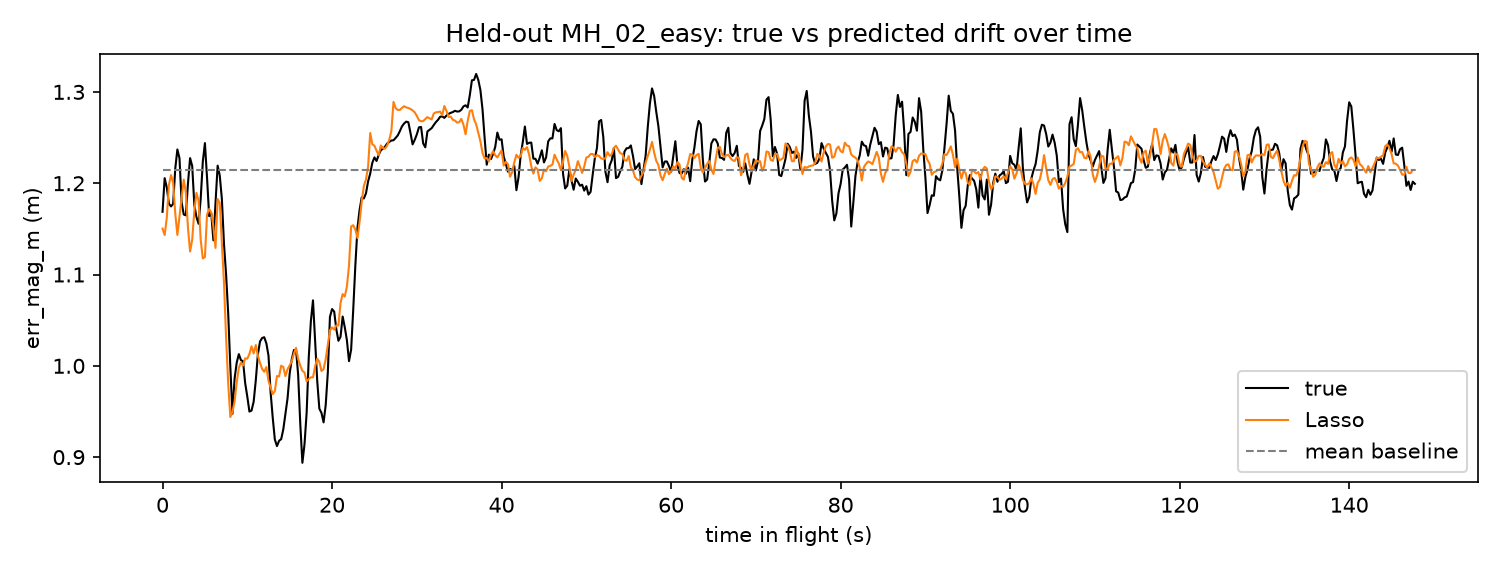
\includegraphics[width=\linewidth]{../../figures/ml/drift_over_time_MH_02_easy.png}
\caption{True drift and Lasso's prediction over the held-out MH\_02\_easy
flight (trained on MH\_01\_easy). Lasso follows the large take-off dip in the
first $\sim$25\,s, but in normal flight its prediction is much smoother than
the truth.}
\label{fig:drift-over-time}
\end{figure}

\subsection{Choosing $\alpha$}
\label{sec:tuning-results}

% Source: results/metrics/err_mag_m.csv (column alpha)
The median rule chose $\alpha = 316$ (trained on MH\_02) and $31.6$ (trained on
MH\_01) for Ridge, and $\alpha = 0.0022$ and $0.00046$ for Lasso.

% Source: results/diagnostics/alpha_sweep_err_mag_m.csv
To check these choices we swept $\alpha$ over the whole grid and scored the
\emph{test} flights (Figure~\ref{fig:alpha-sweep}). This uses test data, so it
is a diagnostic only and played no part in the choice. The curves show the
expected trade-off: at small $\alpha$ the model is essentially OLS, with low
training error but high held-out error; at large $\alpha$ every weight is
pushed to zero and the model becomes the mean baseline. The held-out minimum
lies at $\alpha \approx 100$--$300$ for Ridge and
$\alpha \approx 0.002$--$0.005$ for Lasso on both flights. All four chosen
values fall in the low part of these curves.

\begin{figure}[htbp]
\centering
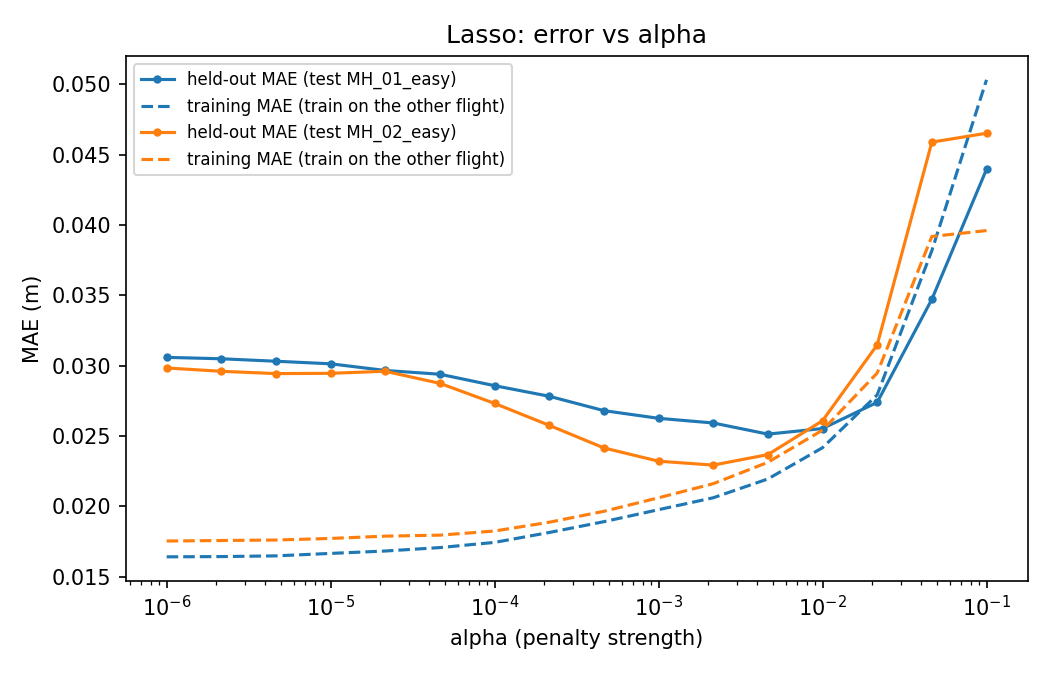
\includegraphics[width=0.8\linewidth]{../../figures/ml/alpha_sweep_lasso.png}
\caption{Lasso training and held-out MAE against $\alpha$, for both folds
(diagnostic only; $\alpha$ is not chosen from this). Ridge shows the same
shape (\texttt{figures/ml/alpha\_sweep\_ridge.png}).}
\label{fig:alpha-sweep}
\end{figure}

% Source: results/diagnostics/tuning_check_err_mag_m.csv (n_blocks = 5)
The median rule matters. With the same 5 blocks, the usual mean rule, trained
on MH\_01, chose Ridge $\alpha = 3.2 \times 10^4$ (held-out $R^2 = 0.32$ instead
of 0.80). The one-standard-error rule was worse: it chose the largest $\alpha$
in the grid for both Ridge ($R^2 = 0.13$) and Lasso, where $\alpha = 0.1$ zeroes
every weight ($R^2 = -0.02$). Trained on MH\_02, all three rules gave good
choices. With 3, 5, 8 or 10 blocks, the median rule never chose an $\alpha$
that zeroes every Lasso weight; with 5 or more blocks it gave Lasso
$R^2 = 0.68$ on MH\_01 and 0.84--0.85 on MH\_02. Tuning on a single flight
remains noisy, though: the median curve itself is bumpy (notebook~05).

\subsection{Over-fitting}
\label{sec:overfitting}

% Source: results/metrics/err_mag_m.csv (columns train_mae, mae, "mean" rows)
\begin{table}[htbp]
\centering
\caption{Training vs.\ held-out MAE, mean of the two folds.}
\label{tab:overfit}
\begin{tabular}{lrrr}
\hline
Model & Train MAE (cm) & Held-out MAE (cm) & Held-out / train \\
\hline
Mean baseline & 4.50 & 4.53 & 1.01 \\
OLS           & 1.65 & 2.99 & 1.81 \\
Ridge (L2)    & 1.95 & 2.70 & 1.38 \\
Lasso (L1)    & 2.01 & 2.50 & 1.24 \\
\hline
\end{tabular}
\end{table}

OLS fits its training flight almost twice as well as the new flight
(Table~\ref{tab:overfit}): with 104 correlated features and about 600 windows
it learns flight-specific noise. The penalties trade a slightly worse training
fit for a clearly better held-out one: the held-out/train ratio falls from 1.81
to 1.38 (Ridge) and 1.24 (Lasso). Lasso does this with few features: it keeps
18 of the 104 when trained on MH\_02 and 40 when trained on MH\_01, and 9 are
kept in both folds, including the accelerometer means and RMS, which encode
the window's tilt against gravity (notebook~05).

\subsection{What the models capture}
\label{sec:segments}

% Source: notebooks/06_model_evaluation.ipynb, Section 5
\begin{table}[htbp]
\centering
\caption{Lasso's held-out $R^2$ and MAE in the first 20\% of each flight
(take-off) and in the remaining 80\%, with the mean baseline's MAE.}
\label{tab:segments}
\begin{tabular}{llrrr}
\hline
Test flight & Part & Lasso $R^2$ & Lasso MAE (cm) & Baseline MAE (cm) \\
\hline
MH\_01 & first 20\% & 0.86 & 2.85 & 8.77 \\
       & remaining 80\% & 0.10 & 2.53 & 3.30 \\
MH\_02 & first 20\% & 0.84 & 3.60 & 13.03 \\
       & remaining 80\% & 0.17 & 2.12 & 2.57 \\
\hline
\end{tabular}
\end{table}

The $R^2$ in Table~\ref{tab:heldout} has to be read with care. Most of a
flight's drift variation is the take-off dip, from about 1.22\,m down to about
1.0\,m (Figure~\ref{fig:drift-over-time}). The models track this slow, large
change well: Lasso reaches $R^2 = 0.84$--$0.86$ in the first 20\% of each
flight (Table~\ref{tab:segments}), and that segment dominates the whole-flight
$R^2$. In normal flight Lasso explains only a small part of the fast
window-to-window changes ($R^2 = 0.10$--$0.17$); its predictions are much
smoother than the truth. It still beats the baseline there in MAE (2.53 vs
3.30\,cm on MH\_01, 2.12 vs 2.57\,cm on MH\_02). Ridge and OLS show the same
pattern ($R^2$ 0.50--0.77 in the first 20\%, $-0.17$ to 0.11 in the rest).

\subsection{Window length}
\label{sec:window-length}

% Source: results/diagnostics/window_length_ceiling.csv (target err_mag_m,
% mean of the two test flights)
\begin{table}[htbp]
\centering
\caption{Mean held-out $R^2$ of \texttt{err\_mag\_m} over the two folds, by
window length, for bias-based predictors.}
\label{tab:window-length}
\begin{tabular}{lrrrr}
\hline
Window length & 0.5\,s & 1\,s & 1.5\,s & 2\,s \\
\hline
Physics feature, no fitting & 0.06 & 0.47 & 0.70 & 0.82 \\
Physics feature, linear fit & 0.13 & 0.48 & 0.70 & 0.82 \\
Oracle ceiling (true bias)  & 0.15 & 0.51 & 0.72 & 0.83 \\
\hline
\end{tabular}
\end{table}

The first version of this pipeline used 1\,s windows. Because the raw label is
mostly integrated bias, whose position error grows quickly with time, while the
rest behaves like noise from window to window, a longer window should make the
label more predictable. To test this without rebuilding the 104 features, every
flight was re-windowed at 0.5--2\,s and scored with three bias-based
predictors (Table~\ref{tab:window-length}): the physics feature
\texttt{phys\_mag} used directly (Section~\ref{sec:physics-feature}); a linear
fit $y \approx a + c \cdot \texttt{phys\_mag}$ on the training flight; and an
\emph{oracle} fit on the test flight's own drift from its true bias, which no
real model can know and which bounds what a bias-based predictor can reach.
All three rise steadily with window length; at 1\,s even the oracle explains
only about half of the variation, against 0.83 at 2\,s. This is why the window
was changed to 2\,s.

The table also shows that the physics feature alone, with no fitting, reaches
$R^2 = 0.82$ at 2\,s, above Lasso's 0.76 on the 104 motion features
(Table~\ref{tab:heldout}). Adding it to the models is the obvious next step.
Like the label, it uses the ground-truth state at the start of each window.

\subsection{Limitations}

With only two flights, every result rests on two folds, and each model is tuned
on a single flight. Both flights are ``easy'' Machine Hall sequences with the
same sensor, so the results say nothing yet about faster or more aggressive
flights. And as Section~\ref{sec:segments} shows, much of the explained
variation comes from the take-off.
